%%
%% This is file `main.tex' based on `sample-sigconf.tex' (q.v. for spurce of that,
%%
%% IMPORTANT NOTICE:
%% 
%% For the copyright see the original source file `sample-sigconf.tex'
%% in the `Sample' folder.
%%
%% For distribution of the original source see the terms
%% for copying and modification in the file samples.dtx.
%% 
%% This generated file may be distributed as long as the
%% original source files, as listed above, are part of the
%% same distribution. (The sources need not necessarily be
%% in the same archive or directory.)
%%
%% Commands for TeXCount
%TC:macro \cite [option:text,text]
%TC:macro \citep [option:text,text]
%TC:macro \citet [option:text,text]
%TC:envir table 0 1
%TC:envir table* 0 1
%TC:envir tabular [ignore] word
%TC:envir displaymath 0 word
%TC:envir math 0 word
%TC:envir comment 0 0
%%
%%
%% The first command in your LaTeX source must be the \documentclass command.
%% NOTE that a single column version is required for 
%% submission and peer review. This can be done by changing
%% the \doucmentclass[...]{acmart} in this template to 
%%\documentclass[manuscript,review,anonymous]{acmart}
%% This version is used for drafting and final submission
\documentclass[sigconf]{acmart}
\usepackage{listings}
\lstdefinestyle{mystyle}{basicstyle=\ttfamily,breaklines=true}

%% To ensure 100% compatibility, please check the white list of
%% approved LaTeX packages to be used with the Master Article Template at
%% https://www.acm.org/publications/taps/whitelist-of-latex-packages 
%% before creating your document. The white list page provides 
%% information on how to submit additional LaTeX packages for 
%% review and adoption.
%% Fonts used in the template cannot be substituted; margin 
%% adjustments are not allowed.

%%
%% \BibTeX command to typeset BibTeX logo in the docs
\AtBeginDocument{%
  \providecommand\BibTeX{{%
    \normalfont B\kern-0.5em{\scshape i\kern-0.25em b}\kern-0.8em\TeX}}}

%% Rights management information.  This information is sent to you
%% when you complete the rights form.  These commands have SAMPLE
%% values in them; it is your responsibility as an author to replace
%% the commands and values with those provided to you when you
%% complete the rights form.
% \setcopyright{acmlicensed}
% \copyrightyear{2024}
% \acmYear{2024}
% \acmDOI{XXXXXX1}

%% These commands are for a PROCEEDINGS abstract or paper.
\acmConference[CUG25]{}{May 4 – May 8, 2025}{Stony Brook, NY}
%
%  Uncomment \acmBooktitle if th title of the proceedings is different
%  from ``Proceedings of ...''!
%
% \acmBooktitle{Woodstock '18: ACM Symposium on Neural Gaze Detection,
%  June 03--05, 2018, Woodstock, NY} 
% \acmISBN{978-1-4503-XXXX-X/18/06}


%%
%% Submission ID.
%% Use this when submitting an article to a sponsored event. You'll
%% receive a unique submission ID from the organizers
%% of the event, and this ID should be used as the parameter to this command.
%\acmSubmissionID{123-A56-BU3}

%%
%% For managing citations, it is recommended to use bibliography
%% files in BibTeX format.
%%
%% You can then either use BibTeX with the ACM-Reference-Format style,
%% or BibLaTeX with the acmnumeric or acmauthoryear sytles, that include
%% support for advanced citation of software artefact from the
%% biblatex-software package, also separately available on CTAN.
%%
%% Look at the sample-*-biblatex.tex files for templates showcasing
%% the biblatex styles.
%%

%%
%% The majority of ACM publications use numbered citations and
%% references.  The command \citestyle{authoryear} switches to the
%% "author year" style.
%%
%% If you are preparing content for an event
%% sponsored by ACM SIGGRAPH, you must use the "author year" style of
%% citations and references.
%% Uncommenting
%% the next command will enable that style.
%%\citestyle{acmauthoryear}

%%
%% end of the preamble, start of the body of the document source.

%% % Location of your graphics files for figures, here a sub-folder to the main project folder
\graphicspath{{./images/}} 


\begin{document}

%%
%% The "title" command has an optional parameter,
%% allowing the author to define a "short title" to be used in page headers.
\title{HPC workload characterization using eBPF}

%%
%% The "author" command and its associated commands are used to define
%% the authors and their affiliations.
%% Of note is the shared affiliation of the first two authors, and the
%% "authornote" and "authornotemark" commands
%% used to denote shared contribution to the research.

\author{Shubh Pachchigar}
\affiliation{%
  \institution{NERSC, Berkeley Lab}}
\email{snpachchigar@lbl.gov}

\author{Brian Friesen}
\affiliation{%
  \institution{NERSC, Berkeley Lab}}
\email{bfriesen@lbl.gov}

\author{Brandon Cook}
\affiliation{%
  \institution{NERSC, Berkeley Lab}}
\email{bgcook@lbl.gov}
%%
%% By default, the full list of authors will be used in the page
%% headers. Often, this list is too long, and will overlap
%% other information printed in the page headers. This command allows
%% the author to define a more concise list
%% of authors' names for this purpose.
\renewcommand{\shortauthors}{Pachchigar et al.}

%%
%% The abstract is a short summary of the work to be presented in the
%% article.
\begin{abstract}

Efficient interactions with filesystems are essential for scientific workflows operating at scale on HPC systems.
In order to design new filesystems, tune system configurations or identify applications for optimization efforts, effective I/O characterization is needed.
Darshan is a widely used tool for I/O characterization that relies on injecting code into application binaries but has some limitations in providing low-level insights.
In this work, we propose leveraging eBPF, a relatively new kernel technology that enables the execution of user-defined programs within the kernel, to develop a new I/O characterization tool. Our approach aims to complement the capabilities of Darshan by using eBPF to gain deeper insight into application interactions with the underlying filesystems. This is achieved by deploying dynamic instrumentation techniques such as tracepoints, kernel probes, and user probes below the application layer to extract detailed I/O metrics.
In this work, we demonstrate the collection of many HPC I/O metrics of various filesystems at NERSC.
The metrics are periodically collected and exposed via a pinned eBPF map with a custom LDMS sampler.
The use of LDMS allows for the collection of data at scale for further processing and analysis.
Finally, to demonstrate its feasibility in production HPC environments, we establish that the overhead of the tool is low.
This work demonstrates the potential of eBPF to enhance I/O characterization in HPC environments, providing valuable insights that can lead to improved performance and resource utilization.

\end{abstract}

%%
%% The code below is generated by the tool at: http://dl.acm.org/ccs.cfm
%% Please copy and paste the code instead of the example below.
%%


%%
%% Keywords. The author(s) should pick words that accurately describe
%% the work being presented. Separate the keywords with commas.
\keywords{eBPF, Darshan, LDMS, HPC, Filesystem, Linux}

%%
%% This command processes the author and affiliation and title
%% information and builds the first part of the formatted document.
\maketitle

\section{Introduction}
High performance scientific workflows have a wide spectrum of I/O patterns\cite{bez2023io}.
At NERSC, there are several network filesystems that a workflow running at scale might interact with: Global common for read-only software, Global homes, Community (CFS) and platform Scratch. 
An efficient interaction with these filesystems, especially in large-scale environments using MPI-IO, POSIX or other interfaces, is important for maximizing workflow performance.
In order to understand and improve the I/O of bare metal or containerized workflows and inform or tune the design of future filesystems, effective characterization of the I/O patterns is essential.

Darshan\cite{snyder2016modular} is a mature HPC I/O characterization tool that provides insights into the I/O behavior of applications running on HPC systems. It generates summaries of I/O activity, including counters, histograms, timers, statistics, and full I/O traces. It is widely adopted across HPC facilities and its modular design allows easy extension to new I/O interfaces and storage components, making it adaptable to evolving storage technologies. However, there are concerns with Darshan modifying binary executables and injecting custom code for instrumentation. There are also potential inaccuracies. For example, Darshan does not understand the notion of virtual and physical memory pages, or caching mechanisms in filesystems or device drivers. 

Extended Berkeley Packet Filter (eBPF) \cite{fleming2017ebpf} is a new technology originating in the Linux kernel that allows sandboxed programs to run in privileged contexts, such as the kernel, without modifying kernel source code or loading kernel modules. It enables developers to extend the kernel’s capabilities safely and efficiently at runtime. eBPF programs are primarily written using three tools: libbpf \cite{nakryiko2022libbpf}, bcc \cite{fleming2017bcc}, and bpftrace \cite{bpftrace_github}. Each operates on a different level of abstraction, bpftrace being the highest and libbpf the lowest and more powerful.

To explore the power of eBPF in workload characterization, we developed several programs using BCC which leveraged different kernel instrumentation techniques, such as user probes on shared objects, tracepoints on the syscall interface, and kernel probes on the VFS to trace application calls. The goal was to understand how the application interacts with different filesystems over time. However, this association proved to be complex, requiring multi-level pointer chasing within internal kernel structures. We discuss this challenge and other findings in more detail later.

We then use Lightweight Distributed Metric Service (LDMS) \cite{ldms}, which is a low-overhead, low-latency framework for collecting, transferring, and storing metric data and is widely used in many HPC centers. In this work, we also explore how to sample eBPF maps directly with a custom LDMS sampler and transport them to an LDMS aggregator for further processing in the pipeline. This approach was chosen to minimize the impact on the system while reusing existing infrastructure. The eBPF programs dump metrics into a special file, which is regularly sampled by LDMS, which then pushes the data to the aggregator.

The rest of the paper is structured as follows: we begin with the implementation of both the eBPF programs and the LDMS samplers, followed by the methodology and setup. Then, we discuss the overhead and present the results.

\begin{figure}
    \centering
    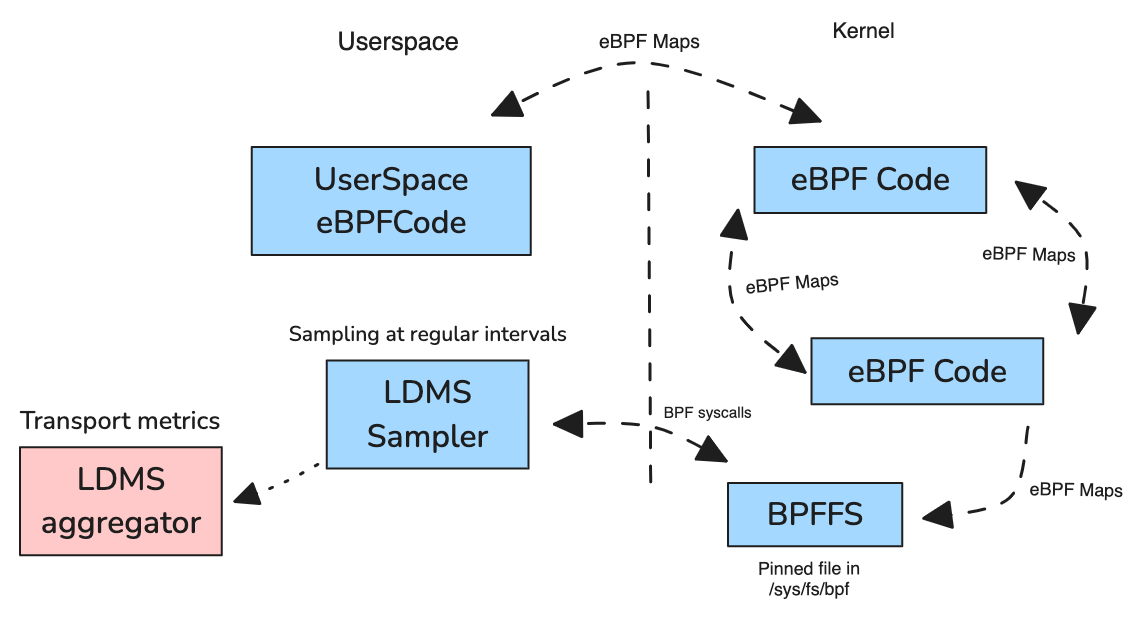
\includegraphics[width=0.45\textwidth]{images/arch.png}
    \caption{Software Architecture}
    \label{fig:arch}
\end{figure}

\section{Implementation}
In this section, we present the implementation details of two important components and explain how they work together. The first subsection provides pseudocode and necessary plots for generating the eBPF programs, while the second subsection describes the technical details of the LDMS sampler and its integration with eBPF. Figure \ref{fig:arch} illustrates the overall architecture, and subsequent subsections will cover each component in detail.

\subsection{eBPF programs} 


Three eBPF programs \cite{ebpf_github} were developed using BPF Compiler Collection (BCC), each targeting different layers of the HPC I/O stack using different kernel instrumentation techniques.

In the first eBPF program, we use uprobes — software breakpoints that enable dynamic instrumentation of arbitrary instructions or symbols within the userspace. Specifically, we target the MPI-IO routines provided by the OpenMPI library. Since the application under analysis links to this library as a shared dependency, these probes allow us to monitor the invocation of MPI-IO symbols in real time. This approach provides valuable insights into the usage patterns and argument values associated with MPI-IO function calls.

In the second program, we utilize kernel tracepoints—lightweight instrumentation hooks placed at strategic locations within the kernel code. Here, we attach tracepoints to the syscall interface to monitor the number of I/O-related calls made to the kernel. An eBPF map is used to store a \texttt{struct}, where the key corresponds to the process identifier (PID), and the value tracks the count of I/O calls issued by that process that reaches the kernel. For each \texttt{sys\_enter} event corresponding to either a \texttt{read} or \texttt{write} operation—whether invoked through MPI-IO or any POSIX-compliant call, we wait for the corresponding \texttt{sys\_exit} event. A successful exit indicates that the I/O operation completed correctly. This mechanism allows us to infer the presence of caching mechanisms in userspace above the kernel layer. Consequently, we can estimate the latency as seen from this level, effectively capturing the delay from one layer to the next in the I/O stack.

\begin{lstlisting}[caption={BPF code: take pointer to struct file and move around kernel structs to get desired information.},label={listing:bpf-basic}, name=bpf-basic, float=h, style=mystyle,language=C++]
struct fs_stat_t {
    char fstype[16];
    char mountpoint[DNAME_INLINE_LEN];
};

static int trace_rw_entry(struct pt_regs *ctx, struct file *file, char __user *buf, size_t count)
{
    struct path p = file->f_path;
    struct vfsmount *vmnt;
    bpf_probe_read_kernel(&vmnt, sizeof(vmnt), &p.mnt);
    struct mount *real_mnt = containerof(vmnt, struct mount, mnt);
    bpf_probe_read_kernel(&fs_info.mnt_id, sizeof(fs_info.mnt_id), &real_mnt->mnt_id);
    struct dentry *m_mp;
    bpf_probe_read_kernel(&m_mp, sizeof(m_mp), &real_mnt->mnt_mountpoint);
    struct qstr m_dname;
    bpf_probe_read_kernel(&m_dname, sizeof(m_dname), &m_mp->d_name);
    bpf_probe_read_kernel(&fs_info.mountpoint, sizeof(fs_info.mountpoint), m_dname.name);
    return 0;
}
\end{lstlisting}
In the third program, we use kernel probes (kprobes), which are special breakpoints inserted into the kernel code. We attach kprobes at the Virtual File System (VFS) layer, specifically targeting the \texttt{vfs\_read} and \texttt{vfs\_write} functions. These probes provide insights into which specific filesystem is being accessed and I/O throughput for that application. The information we store are the filesystem type and the corresponding mount point. The mechanism for extracting this begins with the kprobe on the VFS function, which provides access to a \texttt{struct file}. This structure is the kernel’s primary representation for each an open file, with one instance allocated per open file for MPIIO and POSIX I/O. To determine the filesystem type, we perform a series of pointer dereferences starting from \texttt{struct file}, which points to a \texttt{struct inode}, which in turn points to a \texttt{struct super\_block}, and finally to a \texttt{struct file\_system\_type}. For mount point information, we again begin with \texttt{struct file}, which contains a \texttt{struct path}. \texttt{struct vfsmount} is a member of the \texttt{struct path}, which is also embedded within \texttt{struct mount}. Since we cannot directly get the base address of \texttt{struct mount}, we use the \texttt{container\_of} macro to retrieve its base address. To enable this, we define a minimal version of \texttt{struct mount} within our script. This structure contains the necessary fields to extract mount point information.

All the metrics gathered by the different programs are dumped to a special location in the BPF filesystem. Here, the eBPF maps, which are the primary communication method, are pinned and can only be extracted through the BPF syscall.
\subsection{LDMS sampler and aggregator} 
We have created a new LDMS sampler \cite{ldms_github} that collects metrics generated by eBPF programs in the previous section. These metrics are stored in eBPF maps, which are exported to the BPF filesystem. Since the BPF filesystem resides in kernel space, it can only be accessed via a BPF syscall. As a result, every time the LDMS sampler attempts to collect data, it first makes a BPF syscall to fetch the metrics, then updates its values accordingly.

Typically in LDMS, metrics are created first and then updated during the sampling process. However, in this case, the metric set is dynamic as new buckets or filesystem can be added with each read or write operation. To handle this, we use an LDMS record to initially populate the metric set, storing it in an LDMS list. Each record corresponds to a single metric, with the metric name formed by appending the filesystem name and the corresponding bucket. The value of the metric is either a count or a latency. In addition to the initial record list, a linked list is created to store all the LDMS metrics along with their corresponding LDMS metric IDs. This linked list plays a crucial role in the sampling process. 

During sampling, the first step is to make a BPF syscall atomically in an LDMS transaction to read each entry from the pinned eBPF map. The sampler then checks the linked list to see if the corresponding metric ID already exists. If it does, the value is updated; if not, a new record is created, the value is set, and the record is appended to the existing LDMS list. For this process to work, the final static library for the sampler must be attached to libbpf, which allows the sampler to make the necessary BPF syscalls. Once the sampler is collecting metrics, we can push them to the LDMS aggregator for further post processing.
\begin{figure}
    \centering
    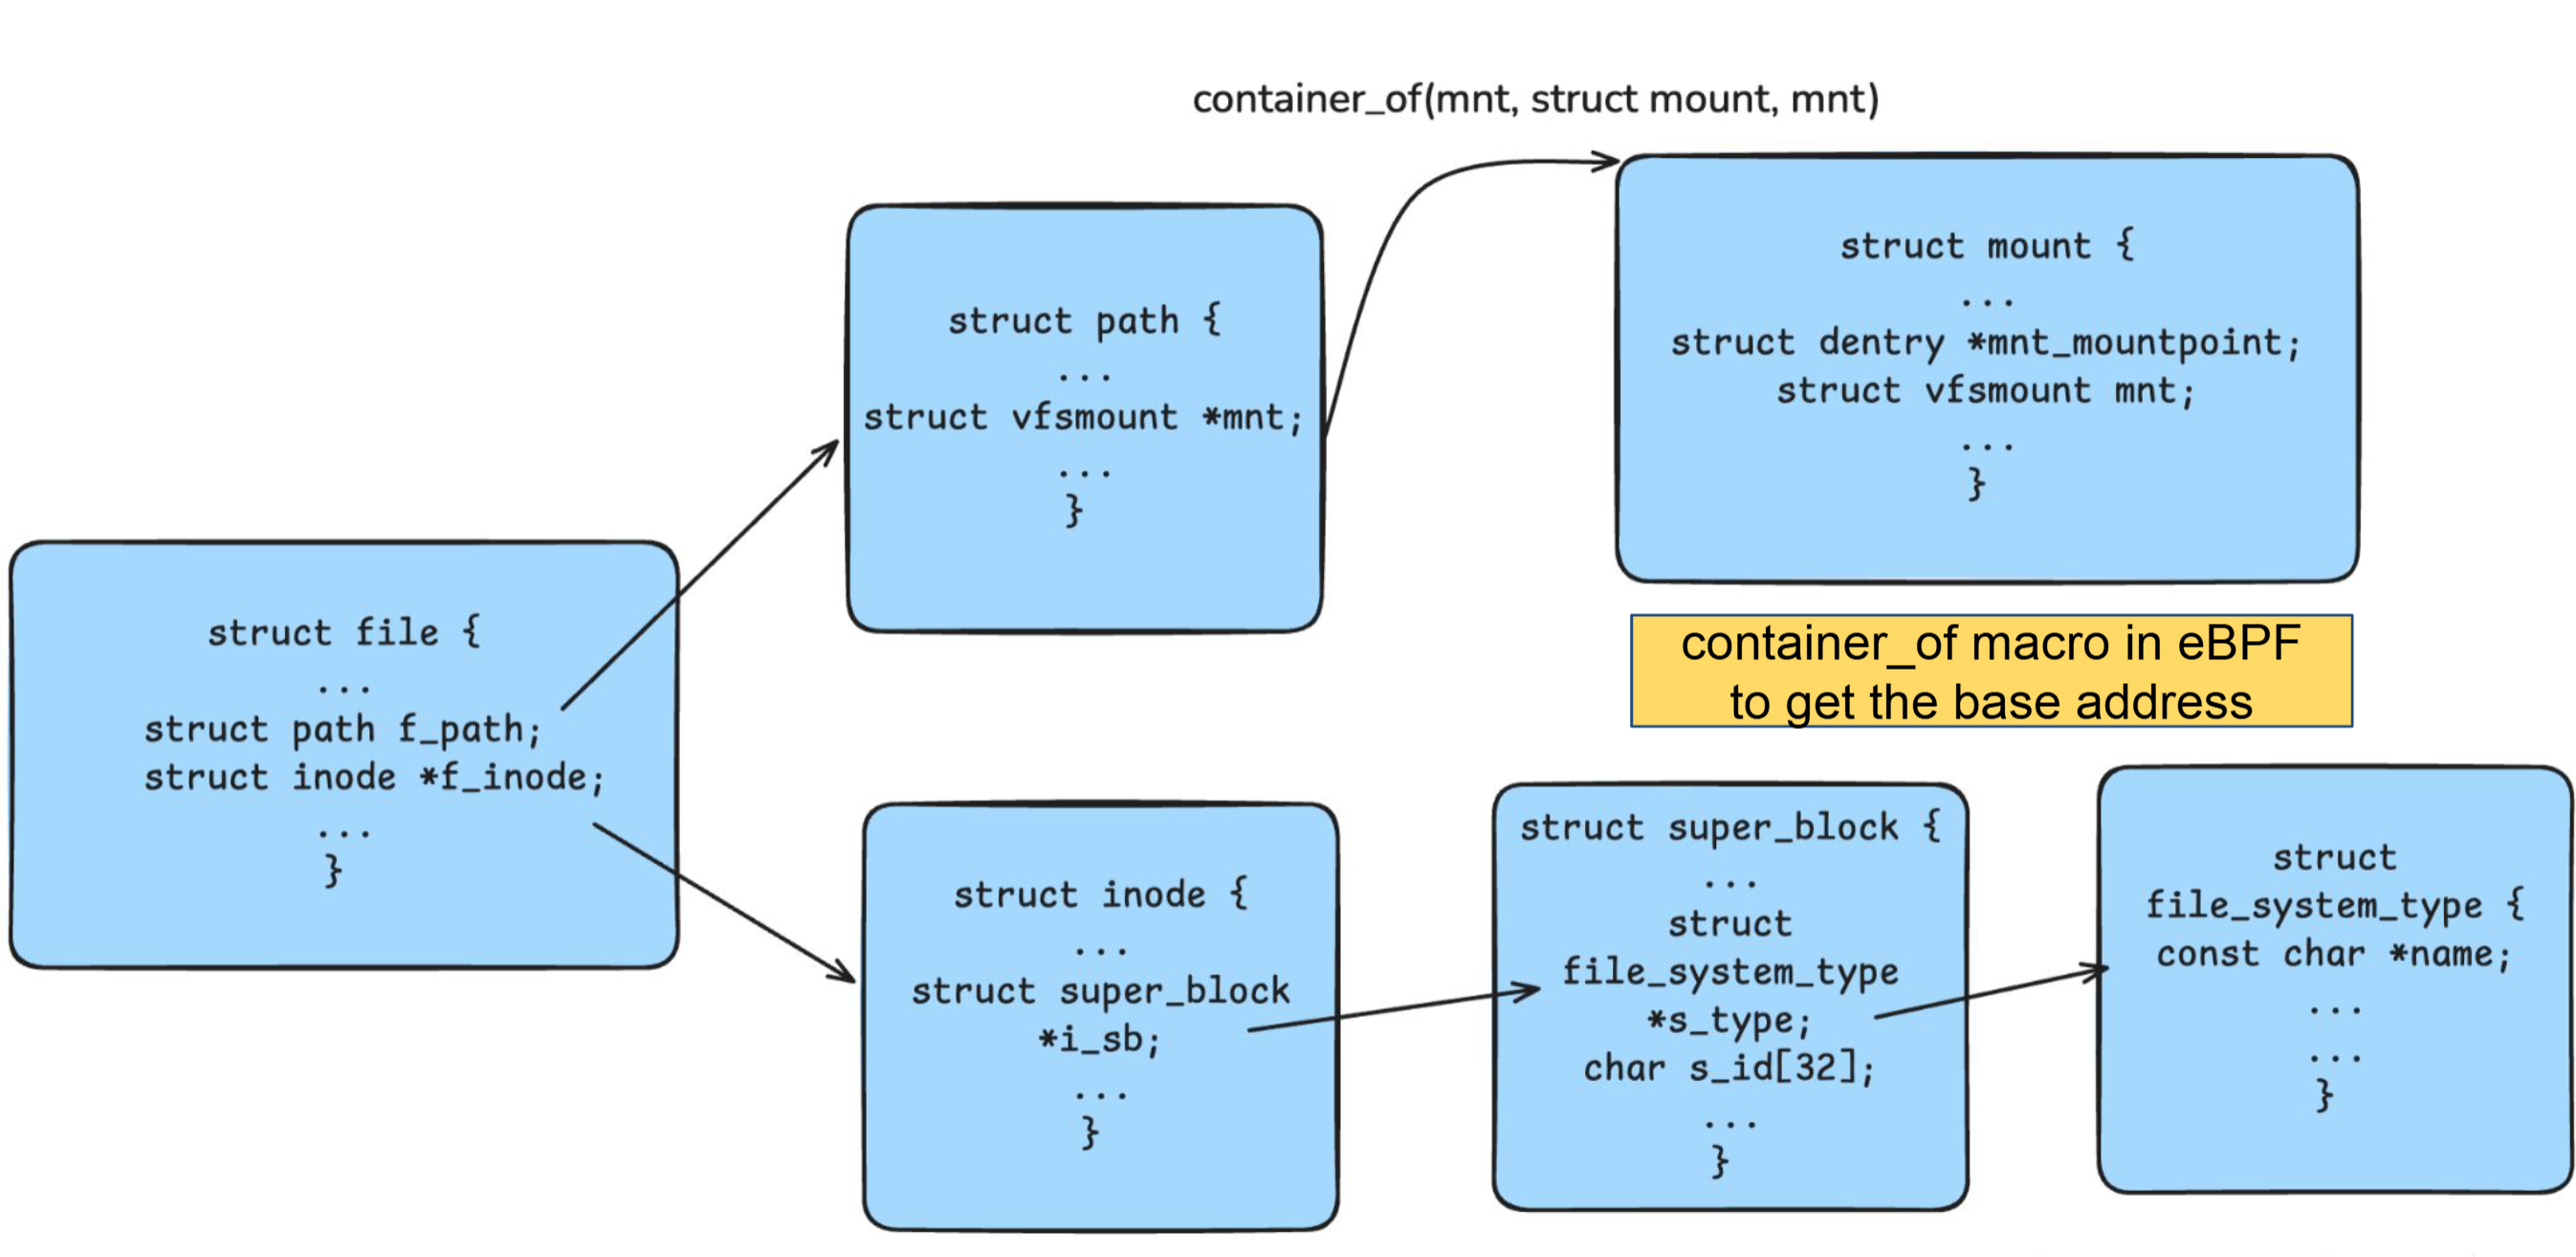
\includegraphics[width=0.45\textwidth]{images/pointer.png}
    \caption{Deep pointer chasing to find filesystem information in Linux}
    \label{fig:pointer}
\end{figure}

\section{Evaluation} 
In this section, we first describe the computation platform and the various software used to implement this work. The initial part will focus on the essential components required to get everything up and running, along with the installation of side dependencies using the default package manager. The second part will then analyze the overhead of the three eBPF programs previously mentioned, within the environment detailed in the next section.

\subsection{Computational platform and Software Environment}
We ran developed our programs on a AWS EC2 instance with OpenSUSE Leap 15.6 and Linux kernel 6.4. For compiling to BPF bytecode, we used Clang 17. Additionally, we installed libbpf 1.5 from source to access all the necessary BPF helpers. We also utilized BCC 0.32 with Python 3.10 and bpftool for inspecting loaded eBPF code and map. We switched from Ubuntu because of some binary stripping causing removal of all symbols and to match production HPC system as closely as possible. For testing, we used Perlmutter TDS (Alvarez) with SUSE Linux Enterprise Server 15 SP5 having a HPE fork of Kernel 5.14. The presence of libclang in \texttt{ld.so.cache} can lead to build errors with eBPF programs. Rebuilding the cache without cray-pe.conf should solve this issue.

\begin{figure}
    \centering
    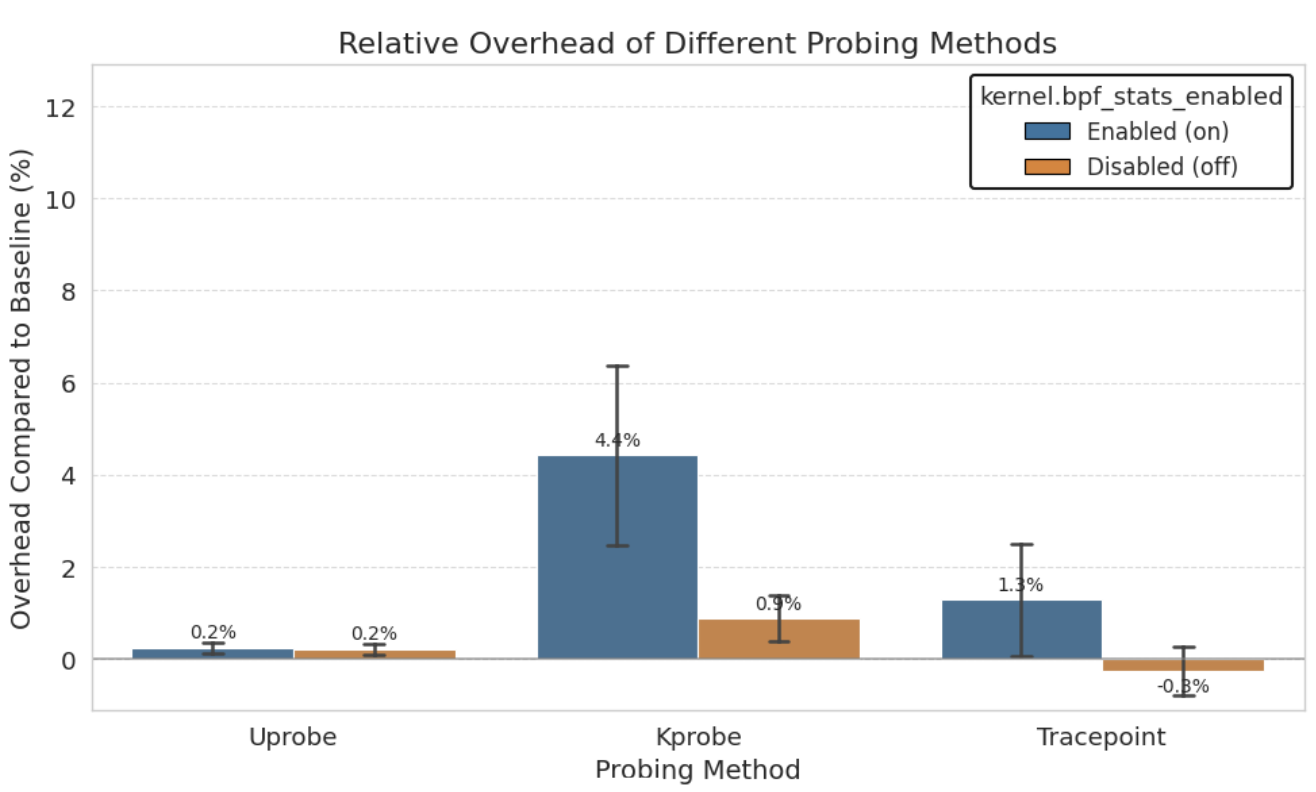
\includegraphics[width=0.45\textwidth]{images/overhead.png}
    \caption{Overhead analysis on EC2 instance}
    \label{fig:overhead}
\end{figure}

\subsection{Overhead anaylsis of eBPF}
There are several ways to measure the overhead of an eBPF script, one of which is by setting \texttt{kernel.bpf\_stats\_enabled = 1}, enabling the tracking of cumulative execution time and the number of invocations of the eBPF program. Overhead can then be calculated as the ratio of total time spent to the number of calls. A comparison of three different kernel dynamic types---Uprobes, Kprobes, and Tracepoints---reveals distinct performance characteristics as shown in the plot above. 

We conducted our experiments on an EC2 instance. We used IOR, configured to operate with MPI-IO. The IOR configuration were kept minimal: sequential I/O operations were performed using two MPI ranks on two physical cores, executing both read and write operations to the xfs filesystem. OpenMPI was used to make the MPIIO calls. To ensure statistical reliability, IOR configuration was executed three times, and the results were averaged to produce a single data point per instrumentation technique. This process was repeated five times to account for variability.

We also evaluated the overhead introduced by enabling the \texttt{sysctl} flag for BPF statistics collection. Specifically, we measure the impact of additional overhead from these runtime statistics for eBPF programs. Our results show that \texttt{uprobes} introduce the least overhead relative to the baseline. This is expected, as MPI-IO calls and their associated subroutines are not frequently invoked by the application or any other process. In contrast, \texttt{kprobes} and \texttt{tracepoints} exhibit slightly higher overheads. This is attributed to the fact that many processes, not just the target application, interact regularly with the kernel and trigger these probes. Interestingly, we observed that \texttt{kprobes} with BPF statistics enabled incurred higher overhead than when BPF statistics were disabled. The exact cause of this difference remains unclear and warrants further investigation. Tracepoints are generally considered lighter-weight than Kprobes \cite{evans_linux_tracing} and which is what we observe as well. Overall we see that overhead of these eBPF programs is mostly in the noise (<5\%) and we are expecting similar results when tested with a real workload on Perlmutter TDS.

\subsection{Results}
The eBPF programs gave expected results when tested on Perlmutter TDS for a simple test application interacting with Lustre and GPFS. The programs are first loaded and corresponding eBPF Maps are pinned to the BPFFS, manually using bpftool. The LDMS sampler then samples the eBPF map for the relevant key and updates the corresponding value. In this case, the number of bytes read/write at the VFS interface, captured by a kprobe, and its associated count are displayed. The key of the map consists of the filesystem type, mountpoint and a log2 bucket, while the value represents the count of I/O operations in that bucket. This demonstrates that the technique is feasible and can be used to gather a much more detailed analysis at a level below the application layer and in the kernel. The LDMS sampler fetches the pinned map and creates a custom key and pushes that to the aggregator nodes.

\section{Conclusion} 
In conclusion, eBPF provides a unique capability to expose the lower layers of systems, allowing us to understand how and through which layers a request passes for I/O operations regardless of if the application runs in containers or bare metal. This capability enables developers and users to perform faster and more detailed analysis. While tools like Darshan work well at the application layer, eBPF can further enhance this analysis, complementing existing methods. We have demonstrated that eBPF programs integrated with LDMS can be deployed in a straightforward manner with minimal changes required on larger HPC systems. The overhead analysis confirms that eBPF introduces a very small proportion of overhead relative to actual application time. Future work will focus on deploying this solution on Perlmutter at NERSC, to assess its impact and overhead in production environments.
%%
%% The acknowledgments section is defined using the "acks" environment
%% (and NOT an unnumbered section). This ensures the proper
%% identification of the section in the article metadata, and the
%% consistent spelling of the heading.
\begin{acks}
This research used resources of the National Energy Research
Scientific Computing Center (NERSC), a U.S. Department of Energy Office of Science User Facility located at Lawrence Berkeley National Laboratory, operated under Contract No. DEAC02-05CH11231.
\end{acks}

%%
%% The next two lines define the bibliography style to be used, and
%% the bibliography file.
\bibliographystyle{ACM-Reference-Format}
\bibliography{references.bib}

%%
\end{document}
\endinput
%%
%% End of file `main.tex'.
